\section{Content}
In this paper, the syntax and typesetting is considered, for building a paper with \LaTeX. By splitting this into sub-files it is easy to work with the project and flexible to change the content without a change of the structure. However, it might be easier to have the structure in another way, once the project evolves. In the following, each example will be defined in the subsection to this \texttt{content} section. Firstly, a short overview of the structure will be given followed by some tests which is carried out as examples of how it is possible to write a descent scientific paper.
%
\input sec/file_structure.tex
%
\subsection{Examples}
\label{sec:examples}
%
\input sec/examples/figures.tex
%
\input sec/examples/math.tex
%
%
%
%
%
%
%
%
%
%
%
%
%
% %
% % Good to have -- for now
% %
%     \begin{figure}[!t]
%     \includegraphics[width=1.5in]{img/jacobm}
%     \caption{caption}
%     \label{fig:label}
%     \end{figure}
% %
% % SUBFIGURE
% %
% And here is a subfigure
% \begin{figure*}[!t]
% \centering
% \subfloat[Case I]{\includegraphics[width=2.5in]{jacobm}%
% \label{fig_first_case}}
% \hfil
% \subfloat[Case II]{\includegraphics[width=2.5in]{jacobm}%
% \label{fig_second_case}}
% \caption{Simulation results.}
% \label{fig_sim}
% \end{figure*}
% 
% %
% % TABLE
% %
% \begin{table}[!t]
% \renewcommand{\arraystretch}{1.3}
% \caption{An Example of a Table}
% \label{table_example}
% \centering
% \begin{tabular}{|c||c|}
% \hline
% One & Two\\
% \hline
% Three & Four\\
% \hline
% \end{tabular}
% \end{table}
